\documentclass[10pt]{article}

\usepackage[paperheight=23 cm, paperwidth=17 cm, top=2 cm, bottom=2 cm, left=2.5 cm, right=1.5 cm]{geometry}
\usepackage[spanish,mexico]{babel}
\usepackage{amsmath} % Some math functions
\usepackage{subcaption} % Subfigures
\usepackage[utf8]{inputenc}
\usepackage{lscape} % Landscape mode
\usepackage[nottoc]{tocbibind} % Include bibliography in TOC

\usepackage[letter,cam,center]{crop} % Crop marks
\usepackage[labelfont=bf]{caption}

\usepackage{graphicx} % OS X

%\usepackage[pdftex]{graphicx} % Windows
%\usepackage{epstopdf} % Windows

%\renewcommand{\baselinestretch}{1.6} %double-spacing

\begin{document}

\thispagestyle{empty}
\tableofcontents
\clearpage

\setcounter{page}{1}

\section{Introducción}

Los mercados de valores permiten el intercambio de activos con facilidad. La mayoría de los estudios de los mercados tratan de explicar el comportamiento de los mismos a través de procesos autorregresivos, en los cuales se trata de explicar la relación del valor actual de una serie de tiempo con los valores anteriores; sin embargo la mayoría de estos estudios ignoran el mecanismo básico detrás de estos mercados: la interacción entre compradores y vendedores.\\

Los mercados se pueden clasificar en dos tipos:
\begin{itemize}
  \item Regidos por formadores de mercado (Quote-driven market)
  \item Regidos por órdenes (Order-driven market)
\end{itemize}

En los mercados regidos por formadores de mercado, éstos centralizan las órdenes proveyendo liquidez al fijar una postura de compra y una venta; por ejemplo el especialista en el NYSE. En los mercados regidos por órdenes, las posturas de todos los participantes se agregan en lo que se conoce como el libro de posturas. Los mercados regidos por órdenes tienen como ventaja la transparencia, ya que todos los participantes conocen las posturas de los demás. Existen algunos mercados híbridos donde los formadores de mercado interactúan en el libro de posturas. La Bolsa Mexicana de Valores y NASDAQ son ejemplos de mercados híbridos.

\clearpage

\section{Descripción de las Base de Datos}
La Bolsa Mexicana de Valores proporcionó para este trabajo una base de datos con las posturas en todas las emisoras entre el 16 de noviembre de 2010 y el 18 de febrero de 2011. La base de datos se compone de dos tablas:

\begin{itemize}
  \item Posturas Iniciales
  \item Registro de Posturas
\end{itemize}

La tabla de registro tiene 25,491,702 renglones; mientras que la tabla de posturas iniciales tiene 275,005. En el registro se encuentran todas las posturas que se reciben a lo largo del día. Las tablas tienen los siguientes campos:\\

\noindent
\begin{tabbing}
\textbf{id} \hspace{3cm} \= Número de identificación \hspace{1cm} \= \\
\\
\textbf{folio} \> Número asignado por la BMV a la postura\\
Según el reglamento de la BMV; las órdenes que, en su caso, tengan modificaciones,\\
perderán el folio de recepción que en un inicio les haya correspondido y se les asignará\\
uno nuevo. No perderán su folio aquellas órdenes que sean modificadas únicamente\\
para disminuir su volumen.\\
\\
\textbf{fecha\_vig/vigencia} \> Fecha de vigencia de la postura \\
\\
\textbf{casabolsa} \> Casa de Bolsa\\
\\
\textbf{tipo\_mov} \> Tipo de Movimiento\\
\underline{Posibles Valores} \\
CO \> Compra\\
VE \> Venta\\
MO \> Modificación\\
CA \> Cancelación\\
AH \> Reconocimiento de Hecho\\
MH \> Modificación de Hecho\\
CH \> Cancelación de Hecho\\
\\
\textbf{tipo\_op} \> Tipo de Operación\\
\underline{Posibles Valores} \\
CO \> Contado\\
PI \> Pico\\
HC \> Operación a Precio de Cierre\\
DC \> Operaciones al Precio de Cierre Modalidad Después del Cierre\\
OR \> Operaciones de Registro\\
OP \> Oferta Pública\\
SR \> Suscripción Recíproca\\
SA \> Sobre Asignación\\
\\
\textbf{tipo\_ord} \> Tipo de Orden\\
\underline{Posibles Valores} \\
LP \> Limitada\\
MC \> Mercado\\
MA \> Mejor Postura Limitada Activa\\
Aquella que sigue el mejor precio límite visible en su mismo sentido y su precio \\
buscará cerrar posturas en sentido contrario que se ubiquen dentro de su precio\\
de protección.\\
MP \> Mejor Postura Limitada Pasiva\\
Aquella que sigue el mejor precio límite visible en su mismo sentido. Aún y cuando\\
existan posturas en sentido contrario dentro de su precio de protección la postura\\
no buscará cerrarlas.\\
VO \> Postura Limitada con Volumen Oculto\\
LO \> Mejor Postura Limitada Activa con Volumen Oculto\\
HC \> Operación a Precio de Cierre\\
DC \> Operaciones al Precio de Cierre Modalidad Después del Cierre\\
PQ \> Paquete \\
\\
\textbf{tipo\_val} \> Tipo de Valor\\
\\
\textbf{emisora} \> Emisora\\
\\
\textbf{serie} \> Serie\\
\\
\textbf{precio} \> Precio\\
\\
\textbf{volumen} \> Volumen\\
\\
La tabla de posturas iniciales utiliza además estos campos:\\
\\
\textbf{fecha} \> Fecha\\
Este campo se utiliza para distinguir las órdenes que están activas al principio del\\
día e inicializar el libro de órdenes.\\
\\
\textbf{orig\_timestamp} \> Fecha original de la postura expresada como la cantidad de\\
\> milésimas de segundo transcurridas desde la medianoche del\\
\>1 de enero de 1970\\
\\
La tabla de registro utiliza estos campos:\\
\\
\textbf{timestamp} \> Fecha de la postura expresada como la cantidad de milésimas\\
\> de segundo transcurridas desde la medianoche del 1 de enero\\
\>de 1970\\
\\
\textbf{folio\_anterior} \> Folio Anterior\\
Se utiliza para localizar el folio de una postura que se va a modificar o cancelar.\\
\\
\textbf{fecha\_folio\_ant} \> Fecha de Folio Anterior\\
\end{tabbing}

\begin{landscape}

\begin{table}[htbp]\scriptsize
\centering
\caption{Posturas Iniciales}
\setlength\tabcolsep{1.5pt}
\begin{tabular}{rrrrrrrrrrrrrr}
\textbf{ id}    & \textbf{fecha} & \textbf{orig\_timestamp} & \textbf{folio} & \textbf{fecha\_vig} & \textbf{tipo\_mov} & \textbf{casabolsa} & \textbf{tipo\_op} & \textbf{tipo\_ord} & \textbf{tipo\_val} & \textbf{emisora} & \textbf{serie} & \textbf{precio} & \textbf{volumen} \\
247 & 24/11/2010 & 1290011934040 & 318480 & 10/12/2010 & CO    & 1277  & CO    & LP    & 1     & LAB   & B     & 25.95 & 2700 \\
292 & 23/11/2010 & 1290189919100 & 368726 & 26/11/2010 & VE    & 1392  & CO    & LP    & 1     & CHDRAUI & B     & 39.8  & 100 \\
519 & 23/12/2010 & 1292863358080 & 242642 & 24/12/2010 & VE    & 1277  & CO    & LP    & 1     & TELMEX & L     & 10.18 & 25000 \\
651 & 27/01/2011 & 1295881813280 & 93317 & 28/01/2011 & VE    & 1664  & CO    & LP    & 1     & ASUR  & B     & 72    & 100 \\
848 & 15/02/2011 & 1295539042060 & 268023 & 18/02/2011 & CO    & 1392  & CO    & LP    & 1     & INCARSO & B-1   & 12.01 & 1000 \\
\ldots & \ldots & \ldots & \ldots & \ldots & \ldots & \ldots & \ldots & \ldots & \ldots & \ldots & \ldots & \ldots & \ldots \\
\end{tabular}%
\label{tab:posinicialesl}%
\end{table}%

\begin{table}[htbp]\scriptsize
\centering
\caption{ Registro de Posturas}
\setlength\tabcolsep{1.5pt}
\begin{tabular}{rrrrrrrrrrrrrrr}
\textbf{ id}    & \textbf{timestamp} & \textbf{folio} & \textbf{vigencia} & \textbf{folio\_anterior} & \textbf{fecha\_folio\_ant} & \textbf{tipo\_mov} & \textbf{casa\_bolsa} & \textbf{tipo\_op} & \textbf{tipo\_ord} & \textbf{tipo\_val} & \textbf{emisora} & \textbf{serie} & \textbf{precio} & \textbf{volumen} \\
48 & 1289916001700 & 19    &       & 0     &       & VE    & 1369  & CO    & LP    & 1     & ARA & *     & 39.6  & 800 \\
329 & 1290785630710 & 124082 & 26/11/2010 & 0     &       & CO    & 1369  & CO    & LP    & 1     & AMX   & L     & 35.69 & 12000 \\
519 & 1291907916550 & 16032 &       & 0     &       & AH    & 1305  & CO    & VO    & 1     & GNP & *     & 58.1  & 1100 \\
652 & 1296246310460 & 911020 &       & 0     &       & VE    & 1369  & PI    & MC    & 1     & ASUR  & B     & 64.05 & 76 \\
998 & 1298062094720 & 566388 & 18/02/2011 & 566388 & 18/02/2011 & MO    & 1288  & CO    & MA    & 1     & BIMBO & A     & 97.51 & 300 \\
\ldots & \ldots & \ldots & \ldots & \ldots & \ldots & \ldots & \ldots & \ldots & \ldots & \ldots & \ldots & \ldots & \ldots & \ldots \\
\end{tabular}%
\label{tab:regposturasl}%
\end{table}%

\end{landscape}

\clearpage

\section{Reconstrucción del Libro de Posturas}

Con los datos proporcionados se reconstruyó el libro de posturas. A lo largo del día existen un gran número de modificaciones y cancelaciones, por lo que para el análisis de los datos es indispensable identificar las posturas activas en cada instante. Aproximadamente el 11\% de los registros en la base de datos son modificaciones, mientras que casi el 35\% son cancelaciones.\\

El algoritmo que se ideó para reconstruir el libro de posturas no toma en cuenta el tipo de orden. Esto se hizo con el fin de simplificar el libro; además de la falta de información como el volumen de las posturas del tipo VO (Volumen Oculto). Las posturas de tipo VO comprenden sólo el 0.55\% del total, mientras que las de tipo LP (Limitadas) representan el 93.81\%. Las operaciones del tipo PI (Picos), las cuales implican la compra/venta de una cantidad de acciones inferior a un lote (para la mayoría de la emisoras son 100 acciones), no se incluyen en el libro de posturas como lo establece el reglamento de la BMV. Las operaciones de tipo PI representan el 0.61\% de la muestra. Adicionalmente como lo establece también el reglamento de la bolsa antes de las 8:30 no se puede concretar ningún hecho, el algoritmo también respeta esto. En primera instancia se cargan las posturas que quedaron abiertas en días anteriores de la tabla de Posturas Iniciales, a continuación se procesa el registro.\\

Para medir la efectividad del algoritmo se compararon los hechos reportados por la BMV con los hechos arrojados por el algoritmo.
Ignorando acciones de muy baja bursatilidad, si se considera la acción de KUO serie B, la cual tiene en promedio alrededor de 28 posturas diarias en la base de datos comparado con la media de 2,550 posturas diarias para las demás emisoras. Para la muestra de 68 días, el algoritmo reproduce el 50.3\% del volumen operado según la BMV. Al analizar el volumen operado con mayor profundidad, esto se debe a una serie de posturas de muy alto volumen que se registraron el 29 de diciembre de 2010. Se puede presumir que se tratan de posturas de volumen oculto. Si se excluye esa fecha el algoritmo reporta un volumen de 5,607,600 acciones mientras que la BMV 5,972,500, es decir el algoritmo registra 6.1\% menos volumen que la bolsa. Para AMX serie L, la acción con mayor volumen en la BMV con un promedio 44,396 posturas por día, el algoritmo reproduce el 89.7\% de las operaciones.\\

Aún más importante que el volumen operado es la tendencia de precios. Una forma de evaluar esto es el VWAP (Volume-weighted average price). El VWAP es el precio promedio ponderado por volumen. Para la acción de KUO el VWAP de por ejemplo el 28 de enero de 2011 registrado por la BMV es de 21.72491, el registrado por el algoritmo es de 21.72289. En un día en donde el volumen operado difiere de mayor forma como el 31 de diciembre de 2010, el VWAP de la bolsa y del algoritmo son similares, 20.35595 y 20.27741 respectivamente. En el caso de AMX, el 28 de diciembre es el día en que el algoritmo reproduce de peor forma el volumen, con un 69.0\% sin embargo la tendencia del precio de las operaciones es bastante similar. El VWAP de las operaciones registradas por la BMV es de 35.12914 mientras que el de el del algoritmo es de 35.10326. Mientras que para el día en el que el algoritmo sigue de mejor forma a las operaciones por la BMV, el 20 de enero de 2011, el VWAP de la bolsa es de 35.28202 mientras que el del algoritmo es de 35.26883.

\begin{figure}[htbp] \centering
\includegraphics[scale=0.75, trim=0 0.5cm 0 1.5cm]{kuo123110.eps}
\caption{Reconstrucción: KUO diciembre 31}
\label{kuo1231}
\end{figure}

\begin{figure}[htbp] \centering
\includegraphics[scale=0.75, trim=0 0.5cm 0 1.5cm]{kuo012811.eps}
\caption{Reconstrucción: KUO enero 28}
\label{kuo0128}
\end{figure}

\begin{figure}[htbp] \centering
\includegraphics[scale=0.75, trim=0 0.5cm 0 1.5cm]{amx012011.eps}
\caption{Reconstrucción: AMX enero 20}
\label{amx0120}
\end{figure}

\begin{figure}[htbp] \centering
\includegraphics[scale=0.75, trim=0 0.5cm 0 1.5cm]{amx122810.eps}
\caption{Reconstrucción: AMX diciembre 28}
\label{amx1228}
\end{figure}

\begin{landscape}

\begin{figure}[htbp] \centering
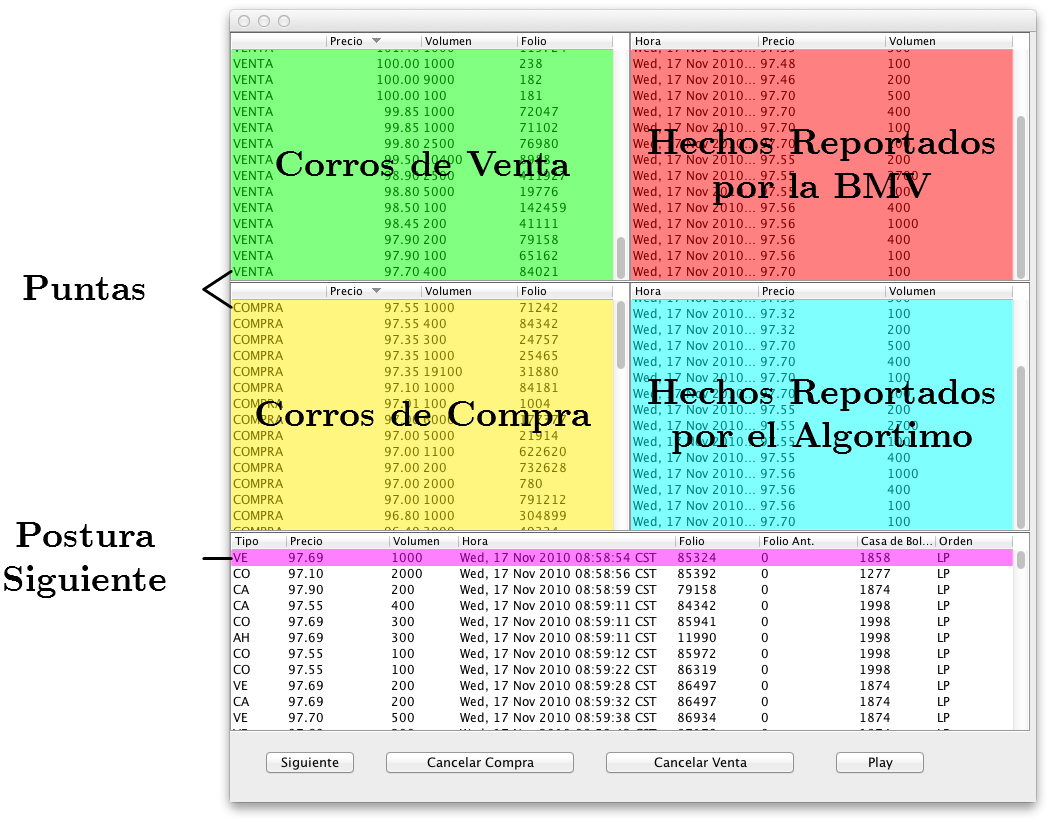
\includegraphics{screenshot.png}
\caption{Captura de pantalla de la Interface desarrollada en Java}
\label{java}
\end{figure}

\end{landscape}

\clearpage

\section{Características Estadísticas del Libro de Posturas}

Los mercados financieros ofrecen un gran número de información, es posible identificar algunos patrones. Por ejemplo se ha identificado que la distribución de los precios de las posturas sigue una ley de potencias, es decir las frecuencias decrecen exponencialmente al aumentar la variable. Es decir si definimos a $b(t)$ como el precio de la mejora postura de compra y $a(t)$ el precio de la mejor postura de venta. El precio de una nueva postura de compra o venta se puede expresar como $b(t)-\Delta$ ó $a(t)+\Delta$ respectivamente, donde la $\Delta$ esta expresada en pujas o ticks, es decir el importe minimo en que puede variar el precio unitario de cada título. Cabe mencionar que $\Delta$ puede tomar valores negativos. Si por ejemplo, con $\Delta <0$, se registra una postura con el precio $b(t)-\Delta \geq a(t)$ entonces se concretará un hecho, mientras que si $b(t)-\Delta < a(t)$ entonces el precio $b(t+1)=b(t)-\Delta$. Ahora si se excluyen las posturas donde $\Delta \leq 0$ se puede decir que los precios siguen una distribución definida por:

\[
P\left(\Delta\right) \propto \frac{A}{{\left(\Delta+\lambda\right)}^{\alpha+1}}
\]\\

Se ajusto el modelo para distintas acciones. Para ajustar el modelo se excluyeron la modificaciones, las cuales se podrían considerar como una nueva postura en algunos casos. Otros estudios han encontrado que el parámetro $alpha$ es muy similar entre las distintas emisoras \cite{zovko2002power} de un mercado en particular, sin embargo, en este caso las acciones tienen parámetros distintos. La distribución ajustada es conocida como Lomax o Pareto Tipo II con $\mu=0$. La media de esta distribución esta definida cuando $\alpha>1$, por lo que en este caso para algunas de las emisoras se podría definir la media. Otro hecho que se destaca en otros trabajos es que el parámetro $\alpha$ es similar para las posturas de compra y venta \cite{Bouchaud2002}. Para las acciones estudiadas en este caso, para una misma emisora el parámetro es similar en la mayoría de los casos, sin embargo, en el caso de KUO el parámetro $\alpha$ para las posturas de venta es 50\% mayor que el de las de compra.

\begin{table}[htbp]
\centering
\caption{Distribución de Precios de las Posturas}
\setlength\tabcolsep{2pt}
\begin{tabular}{r|r|r|r|r|r|r|r|r|r|}
\multicolumn{1}{r}{} & \multicolumn{1}{r}{\textbf{Compra}} & \multicolumn{1}{r}{} & \multicolumn{1}{r}{} & \multicolumn{1}{r}{} & \multicolumn{1}{r}{} & \multicolumn{1}{r}{\textbf{Venta}} & \multicolumn{1}{r}{} & \multicolumn{1}{r}{} & \multicolumn{1}{r}{} \\
\cline{2-5}
\cline{7-10}
& $\lambda$ & $\alpha$ & \#posturas & $\Delta>0$ & & $\lambda$ & $\alpha$ & \#posturas & $\Delta>0$ \\
\cline{2-5}
\cline{7-10}
\textbf{AMX}   & 7.4441 & 1.7098 & 629,302 & 454,039 & & 6.2232 & 1.5022 & 767,215 & 555,595 \\
\textbf{BIMBO} & 14.7809 & 0.8242 & 37,021 & 9,042 & & 31.2291 & 1.2005 & 36,671 & 11,400 \\
\textbf{COMERCI}   & 7.6756 & 1.2256 & 20,955 & 4,201 & & 11.0780 & 1.6555 & 28,893 & 6,584 \\
\textbf{GRUMA} & 58.6601 & 4.4624 & 49,895 & 27,845 & & 63.2991 & 4.1402 & 49,026 & 30,012 \\
\textbf{HERDEZ} & 21.1333 & 2.3332 & 6,811 & 1,773 & & 21.1781 & 2.3215 & 5,493 & 1,263 \\
\textbf{KUO}   & 11.3803 & 0.8556 & 495   & 93    & & 42.1747 & 1.3034 & 319   & 19 \\
\cline{2-5}
\cline{7-10}
\end{tabular}%
\label{tab:power}%
\end{table}%

\begin{figure}[htbp]
\centering
\begin{subfigure}[b]{0.5\textwidth}
\centering
\includegraphics[width=\textwidth, trim=0 0.5cm 0 1cm]{amxcompra.eps}
\caption{AMX compra}
\label{fig:amxcompra}
\end{subfigure}%
~ %add desired spacing between images, e. g. ~, \quad, \qquad etc.
%(or a blank line to force the subfigure onto a new line)
\begin{subfigure}[b]{0.5\textwidth}
\centering
\includegraphics[width=\textwidth, trim=0 0.5cm 0 1cm]{amxventa.eps}
\caption{AMX venta}
\label{fig:amxventa}
\end{subfigure}
%add desired spacing between images, e. g. ~, \quad, \qquad etc.
%(or a blank line to force the subfigure onto a new line)

\begin{subfigure}[b]{0.5\textwidth}
\centering
\includegraphics[width=\textwidth, trim=0 0.5cm 0 1cm]{comercicompra.eps}
\caption{COMERCI compra}
\label{fig:comercicompra}
\end{subfigure}%
~ %add desired spacing between images, e. g. ~, \quad, \qquad etc.
%(or a blank line to force the subfigure onto a new line)
\begin{subfigure}[b]{0.5\textwidth}
\centering
\includegraphics[width=\textwidth, trim=0 0.5cm 0 1cm]{comerciventa.eps}
\caption{COMERCI venta}
\label{fig:comerciventa}
\end{subfigure}
%add desired spacing between images, e. g. ~, \quad, \qquad etc.
%(or a blank line to force the subfigure onto a new line)

\begin{subfigure}[b]{0.5\textwidth}
\centering
\includegraphics[width=\textwidth, trim=0 0.5cm 0 1cm]{kuocompra.eps}
\caption{KUO compra}
\label{fig:kuocompra}
\end{subfigure}%
~ %add desired spacing between images, e. g. ~, \quad, \qquad etc.
%(or a blank line to force the subfigure onto a new line)
\begin{subfigure}[b]{0.5\textwidth}
\centering
\includegraphics[width=\textwidth, trim=0 0.5cm 0 1cm]{kuoventa.eps}
\caption{KUO venta}
\label{fig:kuoventa}
\end{subfigure}
%add desired spacing between images, e. g. ~, \quad, \qquad etc.
%(or a blank line to force the subfigure onto a new line)

\caption{Ajuste del Modelo de Distribución de Precios de las Posturas}\label{fig:fit}
\end{figure}

Se realizó un estudio similar para la distribución del volumen de las posturas. El volumen también se puede representar con una distribución Lomax, por lo menos para volúmenes superiores a 1000 títulos. Otro fenómeno interesante es la preferencia de los participantes por volúmenes múltiplos de 1000.

\clearpage

\section{Modelo del Libro de Posturas Limitado}

Un proceso estocástico $\{X(t);t\geq 0\}$ con un conjunto de estados $\mathcal{S} \subset I$ se dice que es una cadena de Markov homogénea si para toda $n \in I$, estados $i_{0},i_{1},\ldots,i_{n},i,j$ y tiempos $0\leq\tau_0<\tau_1<\cdots<\tau_n<s$

\[
\begin{array}{lcl}
P\{X(t+s)=j|X(\tau_0)=i_0\ldots X(\tau_n)\tau_n)=i_n,X(s)=i\} & = & P\{X(t+s)=j|X(s)=i\} \\
& = & P\{X(t)=j|X(0)=i\}
\end{array}
\]

Un proceso estocástico se conoce como proceso de nacimiento y muerte con un estado de espacios $\mathcal{S}$ si cumple con los siguientes axiomas:

\begin{enumerate}
  \item $\mathcal{S} \subset I = \{ 0,1,2,\ldots\}$
  \item Es una cadena Markov homogénea
  \item Existen las constantes no negativas $\lambda_j$ y $\mu_j$, con $j=0,1,\ldots$ con $\mu_0=0$, tal que para $s>0$ y $t\geq 0$, se cumple:
\begin{equation}
P\{X(t+s)=j+1|X(t)=j\}=\lambda_js + o(s)\quad j \in I 
\end{equation}
\begin{equation}
P\{X(t+s)=j-1|X(t)=j\}=\mu_js + o(s)\quad j \in I 
\end{equation}
\begin{equation}
P\{X(t+s)=j|X(t)=j\}=1-(\lambda_j+\mu_j)s + o(s)\quad j \in I 
\end{equation}
\end{enumerate}

$X(t)$ se conoce como el tamaño de la población al tiempo $t$. A $\lambda_j$ se le conoce como la tasa de nacimiento y $\mu_j$ como la tasa de muerte. Una medida interesante de los procesos de nacimiento y muerte es el tiempo del primer paso del estado {i} al estado {j}, que se denota como $T_{i,j}$. Para calcular la distribución de esta variable aleatoria es conveniente utilizar la transformación de Laplace bilateral. La cual se define de la siguiente forma:

\[
F(s) = \mathcal{L} \left\{f(t)\right\}=\int_{-\infty}^{\infty} e^{-st} f(t) \,dt
\]\\

El tiempo $T_{i,j}$ se puede expresar de la siguiente forma:
\[
T_{i,j}=T_{i,i+1}+T_{i+1,i+2}+\ldots+T_{j-1,j}
\]
donde $T_{k,k+1}$ con $k=1,2,\ldots,j-1$ son independientes, lo cual permite utilizar la siguiente propiedad de la transformación de Laplace:
\[
\hat{f}_{X+Y}(s)=\operatorname{E}[e^{-s(X+Y)}]=\operatorname{E}[e^{-sX}]\operatorname{E}[e^{-sY}]=\hat{f}_{X}(s)\hat{f}_{Y}(s)
\]

Lo cual permite expresar a la transformación de la función de densidad de $T_{i,j}$ como:
\[
\hat{f}_{i,j}(s)=\prod_{k=i}^{j-1}\hat{f}_{k,k+1}(s)
\]
haciendo deseable encontrar una transformación $\mathcal{L}^{-1}$ tal que:
\[
\mathcal{L}^{-1}\{\hat{f}(s)\}=f(t)
\]

Primer es necesario encontrar una expresión para $\hat{f}_{i,i-1}$. Ahora si condicionamos $T_{i,i-1}$ a la primera transición, donde $S_1$ es el tiempo para el primer evento, podemos expresarlo como:

\[
T_{i,i-1} =
\begin{cases}
S_{1}, & \mbox{if } X(S_{1})=i-1 \\
S_{1}+T_{i+1,i-1}, & \mbox{if } X(S_{1})=i+1
\end{cases}
\]
 
\[
T_{i+1,i-1}=T_{i+1,i}+T_{i,i-1}
\]
 
\[
\begin{array}{rcrcl}
F_{i,i-1}(t) & = & P\{ T_{i+1,i-1}\leq t \} & = & P\{ T_{i,i-1}\leq t | X(S_{1})=i-1 \}P\{ X(S_{1})=i-1 \} +\\
 & & & & P\{ T_{i,i-1}\leq t | X(S_{1})=i+1 \}P\{ X(S_{1})=i+1 \} \\
 & & & = & P\{ S_{1}\leq t\}P\{ X(S_{1})=i-1 \} +\\
 & & & & P\{ S_{1} + T_{i+1,i-1}\leq t\}P\{ X(S_{1})=i+1 \} \\
 & & & = & \frac{\mu_{i}}{\lambda_{i}+\mu_{i}} P\{ S_{1}\leq t\} + \frac{\lambda_{i}}{\lambda_{i}+\mu_{i}} P\{ S_{1} + T_{i+1,i-1}\leq t\}\\
 & & & = & \frac{\mu_{i}}{\lambda_{i}+\mu_{i}} F_{S_{1}}(t) + \frac{\lambda_{i}}{\lambda_{i}+\mu_{i}} F_{ S_{1} + T_{i+1,i-1}}(t)\\
\end{array}
\]
 
\[
\begin{array}{rcrcl}
\frac{d}{dt} F_{i,i-1}(t) & = & f_{i,i-1}(t) & = & \frac{\mu_{i}}{\lambda_{i}+\mu_{i}} \frac{d}{dt} F_{S_{1}}(t) + \frac{\lambda_{i}}{\lambda_{i}+\mu_{i}} \frac{d}{dt} F_{ S_{1} + T_{i+1,i-1}}(t)\\
 & & & = & \frac{\mu_{i}}{\lambda_{i}+\mu_{i}} f_{S_{1}}(t) + \frac{\lambda_{i}}{\lambda_{i}+\mu_{i}} f_{ S_{1} + T_{i+1,i-1}}(t)\\
\end{array}
\]

Ahora $S_1$ tiene una distribución exponencial con media $\frac{1}{\lambda_i+\mu_i}$ por lo que:
\[
\mathcal{L}\{f_{S_1}(t)\}=\int_{0}^{\infty} e^{-st} f_{S_1}(t)\,dt=(\lambda_i+\mu_i)\int_{0}^{\infty} e^{-(\lambda_i+\mu_i+s)t}\,dt=\frac{\lambda_i+\mu_i}{\lambda_i+\mu_i+s}
\]

\[
\begin{array}{rcrcl}
\mathcal{L} \{ f_{i,i-1}(t) \} & = & \hat{f}_{i,i-1}(s) & = & \mathcal{L} \{ \frac{\mu_{i}}{\lambda_{i}+\mu_{i}} f_{S_{1}}(t) + \frac{\lambda_{i}}{\lambda_{i}+\mu_{i}} f_{ S_{1} + T_{i+1,i-1}}(t) \}\\
 & & & = & \frac{\mu_{i}}{\lambda_{i}+\mu_{i}} \hat{f}_{S_{1}}(s) + \frac{\lambda_{i}}{\lambda_{i}+\mu_{i}} f_{ S_{1} + T_{i+1,i-1}}(s) \\
 & & & = & \frac{\mu_{i}}{\lambda_{i}+\mu_{i}} \frac{\lambda_{i}+\mu_{i}}{\lambda_{i}+\mu_{i}+s} + \frac{\lambda_{i}}{\lambda_{i}+\mu_{i}} \hat{f}_{S_{1}}(s) \hat{f}_{T_{i+1,i}}(s) \hat{f}_{T_{i,i-1}}(s) \\
 & & & = & \frac{\mu_{i}}{\lambda_{i}+\mu_{i}} \frac{\lambda_{i}+\mu_{i}}{\lambda_{i}+\mu_{i}+s} + \frac{\lambda_{i}}{\lambda_{i}+\mu_{i}} \frac{\lambda_{i}+\mu_{i}}{\lambda_{i}+\mu_{i}+s} \hat{f}_{i+1,i}(s) \hat{f}_{i,i-1}(s) \\
\end{array}
\]
 
\[
\hat{f}_i (s) = \hat{f}_{i,i-1}(s) = \frac{\mu_{i}}{\lambda_{i}+\mu_{i}+s-\lambda_{i}\hat{f}_{i+1}(s)}
\]
\\

Otro concepto que es necesario introducir es lo que se conoce como fracciones continuas. Las cuales son expresiones de la forma:
\[
\cfrac{a_1}{b_1 + 
\cfrac{a_2}{b_2 + 
\cfrac{a_3}{b_3+ \ddots}}}
\]

Una fracción continua infinita se define con las sucesiones $\left[\{a_n\}_1^{\infty},\{b_n\}_1^{\infty},\{w_n\}_1^{\infty}\right]$ donde $t_k$ se define como:
\[
t_k:\rightarrow \frac{a_k}{b_k+u}
\]
donde:
\[
w_n:=t_1\circ t_2 \circ \cdots \circ t_n(0)
\]
por lo que se puede denotar a la fracción continua $\left[\{a_n\}_1^{\infty},\{b_n\}_1^{\infty},\{w_n\}_1^{\infty}\right]$ de la siguiente forma:
\[
\Phi_{k=i}^{\infty}\frac{a_n}{b_n}
\]

Ahora iterando en la expresión que se obtuvo previamente para $\hat{f}_i(s)$, obtenemos:

\[
\hat{f}_i (s) = \cfrac{\mu_{i}}{\lambda_{i}+\mu_{i} + s - \lambda_{i}
\cfrac{\mu_{i+1}}{\lambda_{i+1}+\mu_{i+1} + s - \lambda_{i+1}
\cfrac{\mu_{i+2}}{\lambda_{i+2}+\mu_{i+2} + s + \ddots}}}
\]

\[
\hat{f}_i (s) = -\frac{1}{\lambda_{i-1}} \cfrac{-\lambda_{i-1}\mu_{i}}{\lambda_{i}+\mu_{i} + s +
\cfrac{-\lambda_{i}\mu_{i+1}}{\lambda_{i+1}+\mu_{i+1} + s +
\cfrac{-\lambda_{i+1}\mu_{i+2}}{\lambda_{i+2}+\mu_{i+2} + s + \ddots}}}
\]

\[
\hat{f}_i (s) = -\frac{1}{\lambda_{i-1}}\Phi_{k=i}^{\infty}\frac{-\lambda_{k-1}\mu_{k}}{\lambda_{k}+\mu_{k}+s}
\]
\\

Debido a las propiedades de la función de densidad $f$, se puede probar \cite{abate1999} que $\hat{f}$ converge y esta acotada entre la sucesión creciente de aproximantes pares $w_{2n}$ y la sucesión decreciente de aproximantes impares $w_{2n+1}$:
\[
w_{2n}(s)<\hat{f}(s)<w_{2n+1}(s) \text{ para toda }n 
\]

Donde $w_n$ se puede calcular de la siguiente forma:
\[
w_n=\frac{P_n}{Q_n}
\]
donde $P_0=0, P_1=a_1,Q_0=1,Q_1=b_1$ con:
\[
P_n=b_n P_{n-1}+a_n P_{n-2}
\]
\[
Q_n=b_n Q_{n-1}+a_n Q_{n-2}
\]
\\

El reto que aún queda es encontrar una forma de calcular numéricamente $\mathcal{L}^{-1}$, la cual esta definida por la siguiente integral de variable compleja, la cual se puede evaluar a lo largo de la línea vertical $\gamma=a$, de la siguiente manera:

\[
\begin{array}{rcl}
f(t) = \mathcal{L}^{-1} \{\hat{f}(s)\} & = & \displaystyle \frac{1}{2 \pi i} \lim_{T\to\infty}\int_{ a - i T}^{ a + i T} e^{st} \hat{f}(s)\,ds\\
& = & \displaystyle \frac{1}{2 \pi} \int_{ -\infty}^{ \infty} e^{(a+iu)t} \hat{f}(a+iu)\,du\\
& = & \displaystyle \frac{e^{at}}{2 \pi} \int_{ -\infty}^{ \infty} (cos\,ut + i sin\,ut)\hat{f}(a+iu)\,du\\
& = & \displaystyle \frac{e^{at}}{2 \pi} \int_{ -\infty}^{ \infty} \left[Re(\hat{f}(a+iu))cos\,ut - Im(\hat{f}(a+iu))sin\,ut\right]\,du\\
& = & \displaystyle \frac{2e^{at}}{\pi} \int_{0}^{ \infty} Re(\hat{f}(a+iu))cos\,ut\,du\\
\end{array}
\]

Para evaluar esta integral hacemos uso de la regla del trapecio, con un tamaño de paso $h$, dando como resultado:
\[
f(t)\approx f_h(t)=\frac{he^{at}}{\pi} Re(\hat{f}(a))+\frac{2he^{at}}{\pi}\sum_{k=1}^{\infty}Re(\hat{f}(a+ikh))cos\,kht
\]

Ahora si se toma $h=\pi/2t$ y $a=A/2t$, se llega a la siguiente serie, la cual es casi alternante:

\[
f_h(t)=\frac{e^{A/2}}{2t} Re\left(\hat{f}\left(\frac{A}{2t}\right)\right)+\frac{e^{A/2}}{t}\sum_{k=1}^{\infty}(-1)^k Re\left(\hat{f}\left(\frac{A+2k\pi i}{2t}\right)\right)
\]
esta aproximación tiene un error de discretización acotado \cite{abate1995}.\\

Debido a que la serie es casi alternante se pueden utilizar métodos para acelerar la convergencia, tal como la transformación de Euler. Al utilizar este método obtenemos la siguiente aproximación:
\[
E(m,n,t)=\sum_{k=0}^m \binom mk 2^{-m}s_{n+k}(t)
\]
donde:
\[
s_n=\frac{e^{A/2}}{2t} Re\left(\hat{f}\left(\frac{A}{2t}\right)\right)+\frac{e^{A/2}}{t}\sum_{k=1}^{n}(-1)^k Re\left(\hat{f}\left(\frac{A+2k\pi i}{2t}\right)\right)
\]
\\

En este caso se utiliza $m=11$ y $n=15$. Para probar la ventaja de la aceleración se encontró la transformación de Laplace de la función de densidad de una variable aleatoria con distribución exponencial. La aceleración permite encontrar una aproximación muy cercana sumando 26 términos mientras que cuando no se recurre a este método, el error de aproximación es mayor aún utilizando 2000 términos. Es importante mencionar que las funciones deben de tener ciertas propiedades para que la transformación de Euler sea útil.

\clearpage

\listoftables
\clearpage

\listoffigures
\clearpage

\nocite{*}

\bibliographystyle{apalike}
\bibliography{myrefs}

\end{document}